% ----- Conclusion -----

\section{Conclusion}

As seen in the previous sections, we have been able to implement different
algorithm to solve the Maximum Edge Weight Clique problem. We have also been
able to compare the different algorithms and to determine which one is the most
efficient depending on the number of vertices and the connectivity of the graph.
\bigskip

Since the MEWC problem is NP-hard, it is not possible to find a solution in
polynomial time. We have therefore tried to optimize the solution of the problem
by trying to find the most efficient algorithm to solve the problem in the best
way.
\bigskip

\large\textbf{Comparison of algorithms} \newline 

\underline{Speed of results}\bigskip

We are now going to compare the different algorithms from a general point of view, even if it would be necessary to do a study again according to the starting graph we have.
Let's look at the complexity and the execution time of these different algorithms.

\begin{itemize}
    \item \textbf{Complexity} : As we compare the complexity of the algorithms we obtain : \bigskip
    
Exact (O($n^2\sqrt[3]{3}^n$)) - Constructive (O($n^2$)) - Local Search (O($n^5$)) - Grasp (O($n^6$)) \bigskip
    
    Since the complexity will vary depending on the connectivity and degeneracy of the graph we will look at the execution time too.
    
    \item \textbf{Execution time} : \bigskip
    
Constructive ($5.10^6$) -  Local Search (A COMPLETER) - Grasp ($10^8$) - Exact ($\thicksim 10^8$) 
\end{itemize}
\underline{Accuracy of results}\bigskip 

Another very important criterion to consider is the accuracy of the answer obtained. \bigskip 

Accuracy is in this order (from most to least accurate):

Exact - Grasp - Local Search - Constructive \bigskip 

\large\textbf{Choice of the algorithm} \newline

After this, we decided to conclude according to the number of vertices of our strating graph :

\begin{itemize}
    \item \textbf{10 - 100 Vertices} : We will use the "Exact" algorithm which allows to give a very precise solution but which is slow.

    \item \textbf{100 + Vertices} : In order to don't wait too long for an answer, we plan to use the "Grasp" algorithm and then the "Local Search" which are certainly less precise but which allows to give an answer in less time.

    \item \textbf{5000 + Vertices} : Finally we will use the "Constructive" algorithm which is the least precise but the fastest and allows to answer in an acceptable time

\end{itemize}

\begin{figure}[H]
    \centering
    \begin{tikzpicture}
        \begin{axis}[
                xlabel = Number of vertices,
                ylabel = \% of solution based on exact,
                legend pos = outer north east,
                grid = major,
                width = 0.5\textwidth,
                legend cell align = {left},
            ]
            \addplot[Red, error bars/.cd, y dir=both, y explicit]
            table[x index=0, y index=1] {experiment_data/accuracy_avg_exact.dat};

            \addplot[Green, error bars/.cd, y dir=both, y explicit]
            table[x index=0, y index=1] {experiment_data/accuracy_avg_constructive_25.dat};

            \addplot[Blue, error bars/.cd, y dir=both, y explicit]
            table[x index=0, y index=1] {experiment_data/accuracy_avg_local_search_25.dat};

            \addplot[Black, error bars/.cd, y dir=both, y explicit]
            table[x index=0, y index=1] {experiment_data/accuracy_avg_grasp_25.dat};

            \addlegendentry{test}

            \legend{exact, constructive, local search, grasp}
        \end{axis}
    \end{tikzpicture}
    \caption{\% of solution based on the exact of the different algorithm for 25\% of connectivity.}
    \label{fig:algorithm_25_time}
\end{figure}

For this experiment, we generated 10 random graphs with 10 to 100 vertices to find an
average \% for 25\% of connectivity. The connectivity is the percentage
of chance that 2 vertices are linked. The results are shown in figure \ref{fig:algorithm_25_time}. At each number of
vertices, an average clique weight is calculated, and converted to \% based on the result obtained with the exact algorithm.
// à martin de détailler

\begin{figure}[H]
    \centering
    \begin{tikzpicture}
        \begin{axis}[
            xlabel = Number of vertices,
            ylabel = \% of solution based on exact,
                legend pos = outer north east,
                grid = major,
                width = 0.5\textwidth,
                legend cell align = {left},
            ]
            \addplot[Red, error bars/.cd, y dir=both, y explicit]
            table[x index=0, y index=1] {experiment_data/accuracy_avg_exact.dat};

            \addplot[Green, error bars/.cd, y dir=both, y explicit]
            table[x index=0, y index=1] {experiment_data/accuracy_avg_constructive_50.dat};

            \addplot[Blue, error bars/.cd, y dir=both, y explicit]
            table[x index=0, y index=1] {experiment_data/accuracy_avg_local_search_50.dat};

            \addplot[Black, error bars/.cd, y dir=both, y explicit]
            table[x index=0, y index=1] {experiment_data/accuracy_avg_grasp_50.dat};

            \addlegendentry{test}

            \legend{exact, constructive, local search, grasp}
        \end{axis}
    \end{tikzpicture}
    \caption{\% of solution based on the exact of the different algorithm for 50\% of connectivity.}
    \label{fig:algorithm_50_time}
\end{figure}

For this experiment, we generated 10 random graphs with 10 to 100 vertices to find an
average \% for 50\% of connectivity. The connectivity is the percentage
of chance that 2 vertices are linked. The results are shown in figure \ref{fig:algorithm_50_time}. At each number of
vertices, an average clique weight is calculated, and converted to \% based on the result obtained with the exact algorithm.
// à martin de détailler

\begin{figure}[H]
    \centering
    \begin{tikzpicture}
        \begin{axis}[
            xlabel = Number of vertices,
            ylabel = \% of solution based on the exact,
                legend pos = outer north east,
                grid = major,
                width = 0.5\textwidth,
                legend cell align = {left},
            ]
            \addplot[Red, error bars/.cd, y dir=both, y explicit]
            table[x index=0, y index=1] {experiment_data/accuracy_avg_exact.dat};

            \addplot[Green, error bars/.cd, y dir=both, y explicit]
            table[x index=0, y index=1] {experiment_data/accuracy_avg_constructive_75.dat};

            \addplot[Blue, error bars/.cd, y dir=both, y explicit]
            table[x index=0, y index=1] {experiment_data/accuracy_avg_local_search_75.dat};

            \addplot[Black, error bars/.cd, y dir=both, y explicit]
            table[x index=0, y index=1] {experiment_data/accuracy_avg_grasp_75.dat};

            \addlegendentry{test}

            \legend{exact, constructive, local search, grasp}
        \end{axis}
    \end{tikzpicture}
    \caption{\% of solution based on the exact of the different algorithm for 75\% of connectivity.}
    \label{fig:algorithm_75_time}
\end{figure}

For this experiment, we generated 10 random graphs with 10 to 100 vertices to find an
average \% of clique weight for 75\% of connectivity. The connectivity is the percentage
of chance that 2 vertices are linked. The results are shown in figure \ref{fig:algorithm_75_time}. At each number of
vertices, an average clique weight is calculated, and converted to \% based on the result obtained with the exact algorithm.
// à martin de détailler

\begin{figure}[H]
    \centering
    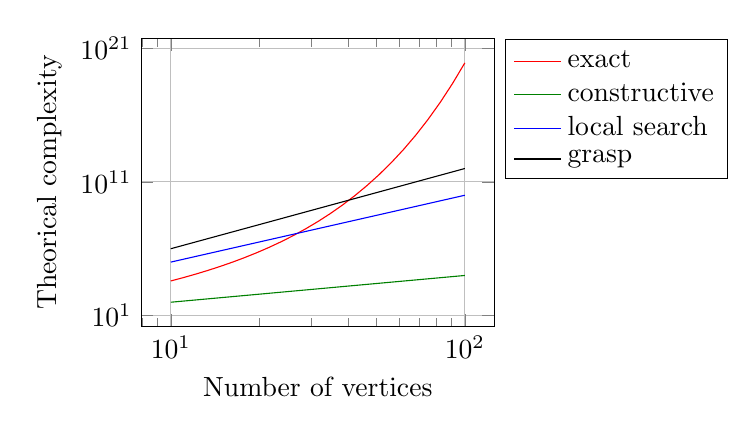
\begin{tikzpicture}
        \begin{loglogaxis}[
                xlabel = Number of vertices,
                ylabel = Theorical complexity,
                legend pos = outer north east,
                grid = major,
                width = 0.5\textwidth,
                legend cell align = {left},
            ]
            \addplot[Red, domain=10:100] {x^2*3^(x/3)};

            \addplot[Green, domain=10:100] {x^2};

            \addplot[Blue, domain=10:100] {x^5};

            \addplot[Black, domain=10:100] {x^6};


            \addlegendentry{test}

            \legend{exact, constructive, local search, grasp}
        \end{loglogaxis}
    \end{tikzpicture}
    \caption{Execution time of the constructive algorithm for different percentages of connectivity.}
    \label{fig:constructive_time}
\end{figure}